\chapter{Over-Approximation and Under-Approximation}\label{chap:OT-UT}
\section{Approximation Theory}
\begin{comment}
$F = \exists x_1 \in I_1 \cdots x_n \in I_n. \bigwedge \limits_j \psi_j(x_1,\cdots,x_n)$, 
%\exists x_1 \ldots x_n. (\underbrace{\bigwedge \limits_i x_i \in I_i}_{I}) \wedge 
%                       (\underbrace{\bigwedge \limits_j \psi_j(x_1,\cdots,x_n)}_{P})
where $\psi_j(x_1,\cdots,x_n)$ is an atomic formula. 
%
$F$ is equivalnet to 
$\exists x_1 \ldots x_n. (\bigwedge \limits_i x_i \in I_i) \wedge (\bigwedge \limits_j \psi_j(x_1,\cdots,x_n))$, 
and we call $\bigwedge \limits_i x_i \in I_i$ {\em interval constraints}, and 
we refer $\bigwedge \limits_j \psi_j(x_1,\cdots,x_n)$ by $\psi(x_1,\cdots,x_n)$. 
Initially, interval constraints have a form of the conjunction $\bigwedge \limits_i x_i \in I_i$, 
and later by refinement, $x_i \in I_i$ is decomposed into a clause $\bigvee_j x_i \in I_{i_j}$, 
which makes a CNF. 

As an SMT (SAT modulo theory) problem, 
boolean variables are assigned to each $x_i \in I_{i_j}$, 
and truth assignments is produced by a SAT solver, 
which are proved or disproved by a background theory $T$ whether it satisfies $\psi(x_1,\cdots,x_n)$. 

As notational convention, $m$ (the lower case) denotes 
a variable assignments on $x_i$'s, and 
$M$ (the upper case) denotes a truth assignment on $x_i \in I_{i_j}$'s. 
We write $m \in M$ when an instance $m = \{ x_i \leftarrow c_i \}$ satisfies 
all $c_i \in I_{i_j}$ that are assigned true by $M$. 

We assume {\em very lazy theory learning}~\cite{dpll}, and 
a backend theory $T$ is applied only for a full truth assignment $M$. 
%We regard $M$ as a conjunction $\bigwedge \limits_i x_i \in I_{i_j}$. 
\begin{itemize}
\item If an instance $m$ satisfies $\psi(x_1,\cdots,x_n)$, we denote $m \models_T \psi(x_1,\cdots,x_n)$. 
\item If each instance $m$ with $m \in M$ satisfies $\psi(x_1,\cdots,x_n)$, 
we denote $M \models_T \psi(x_1,\cdots,x_n)$. 
\end{itemize}
\end{comment}

\begin{comment}
\begin{definition} \label{def:app}
Let $F = \exists x_1 \in I_1 \cdots x_n \in I_n. \psi(x_1,\cdots,x_n)$. 
For a truth assignment on $M$, $F$ is 
\begin{itemize}
\item $T$-valid if $M \models_T \psi(x_1,\cdots,$ $x_n)$, 
\item $T$-satisfiable ($T$-SAT) if $m \models_T \psi(x_1,\cdots,x_n)$ 
for some $m \in M$, and 
\item $T$-unsatisfiable ($T$-UNSAT) if $M \models_T \neg \psi(x_1,\cdots,x_n)$. 
\end{itemize}
If $T$ is clear from the context, we simply say valid, satisfiable, and unsatisfiable. 
\end{definition}
\end{comment}

%%%%%%%%%%%%%
\suppress{
Then, Fig. \ref{fig:T_result} illustrates Definition~\ref{def:app}. 
\begin{figure} [ht]
\centering
\begin{minipage}[b]{0.45\linewidth}
  \includegraphics[height=1.8in,width=1.9in]{T_result.eps}
\caption{Results of a target constraint $F$ in a theory $T$}
\label{fig:T_result}
\end{minipage}
\quad
\begin{minipage}[b]{0.45\linewidth}
   \includegraphics[height=2.2in,width=2.3in]{frame_app.eps}
\caption{{\bf raSAT} loop}
\label{fig:frame}
\end{minipage}
\end{figure}
}
%%%%%%%%%%%%%%%%%%%%%%%%%%%%%%%%

\begin{definition} \label{def:ApproxTheory}
Let $T, T'$ be $\Sigma$-theories and $\varphi$ be any $\Sigma$-formula. 
\begin{itemize}
\item[$\bullet$] $T'$ is an {\em over-approximation theory} of $T$ 
iff $T'$-UNSAT of $\varphi$ implies $T$-UNSAT of $\varphi$.
\item[$\bullet$] $T'$ is an {\em under-approximation theory} of $T$
iff $T'$-SAT of $\varphi$ implies $T$-SAT of $\varphi$. 
\end{itemize}
\end{definition}

\begin{theorem}
If $T_O$ be an over-approximation theory of $T$, then for any $\Sigma$-formula $\varphi$: $\varphi$ is $T_O$-VALID implies $\varphi$ is $T$-VALID.
\end{theorem}

\begin{proof}
$\varphi$ is $T_O$-VALID $\implies$ $\neg\varphi$ is $T_O$-UNSAT (Lemma \ref{lemma:theory-valid-unsat}) $\implies \neg\varphi$ is $T$-UNSAT (Definition \ref{def:ApproxTheory}) $\implies \varphi$ is T-VALID (Lemma \ref{lemma:theory-valid-unsat})
\end{proof}


\section{Interval Arithmetic as an Over-Approximation Theory of Sub-Theory of Real Numbers}\label{sec:IA}
\subsection{Real Intervals}
We adopt the definition of real intervals from \cite{Hickey:2001:IAP:502102.502106}:
\begin{definition}\cite{Hickey:2001:IAP:502102.502106}
Let $a$ and $b$ be reals such that $a \le b$.
\begin{center}
\begin{tabular}{ r c l }
  $\langle a, b \rangle$ & $\overset{def}{=}$ & $\{x \in \mathbb{R} | a \le x \le b\}$ \\
  $\langle -\infty, b \rangle$ & $\overset{def}{=}$ & $\{x \in \mathbb{R} | x \le b\}$ \\
  $\langle a, +\infty \rangle$ & $\overset{def}{=}$ & $\{x \in \mathbb{R} | a \le x\}$ \\  
  $\langle -\infty, +\infty \rangle$ & $\overset{def}{=}$ & $\mathbb{R}$ \\  
\end{tabular}
\end{center}
\end{definition}
The \emph{intervals} in this definition can be summarized by $\langle a, b \rangle$ where $a, b \in \mathbb{R} \cup \{-\infty, +\infty\}$ and $a \le b$ with the assumption that $\forall c \in \mathbb{R}-\infty < c < \infty$. Furthermore,\citet{Hickey:2001:IAP:502102.502106} also defined arithmetic operations for $\mathbb{R} \cup \{-\infty, +\infty\}$ which is summarized in Table~\ref{tab:arithOp}.

\begin{table} \label{tab:arithOp}
\begin{tabular}{c||*{5}{c|}}
$x + y$
&$-\infty$&NR&0
&PR&$+\infty$\\\hline
$-\infty$ &$-\infty$&$-\infty$&$-\infty$&$-\infty$&$\bot$\\\hline
$NR$ &&NR&NR&$\mathbb{R}$&$+\infty$\\\hline
$0$&&&0&PR&$+\infty$\\\hline
$PR$ &&&&PR&$+\infty$\\\hline
$+\infty$ &&&&&$+\infty$\\\hline
\end{tabular}
\quad
\begin{tabular}{c||*{5}{c|}}
$x - y$
&$-\infty$&NR&0
&PR&$+\infty$\\\hline
$-\infty$ &$\bot$&$+\infty$&$+\infty$&$+\infty$&$+\infty$\\\hline
$NR$ &$-\infty$&$\mathbb{R}$&PR&PR&$+\infty$\\\hline
$0$&$-\infty$&NR&0&PR&$+\infty$\\\hline
$PR$ &$-\infty$&NR&NR&$\mathbb{R}$&$+\infty$\\\hline
$+\infty$ &$-\infty$&$-\infty$&$-\infty$&$-\infty$&$\bot$\\\hline
\end{tabular}
\newline
\vspace*{1 cm}
\newline
\begin{center}
\begin{tabular}{c||*{5}{c|}}
$x \times y$
&$-\infty$&NR&0
&PR&$+\infty$\\\hline
$-\infty$ &$+\infty$&$+\infty$&$\bot$&$-\infty$&$-\infty$\\\hline
$NR$ &&PR&0&NR&$-\infty$\\\hline
$0$&&&0&0&$\bot$\\\hline
$PR$ &&&&PR&$+\infty$\\\hline
$+\infty$ &&&&&$+\infty$\\\hline
\end{tabular}
\end{center}
\caption{Arithmetics Operations for $\mathbb{R} \cup \{-\infty, +\infty\}$}
\end{table}

\begin{definition} \label{def:real_intervals}
The set of all \emph{real intervals} $\mathbb{I}$ is defined as: \[\mathbb{I} = \{\langle a, b \rangle | a, b \in \mathbb{R} \cup \{-\infty, +\infty\} \text{ and } a \le b \}\].
\end{definition}

\subsection{Interval Arithmetic as an Over-Approximation Theory of Sub-Theory of Real Numbers} \label{sec:Gen-IA}
\sloppy
A model $M^p_{IA} = (\mathbb{I}, I^p_{IA})$ over intervals for polynomial constraints consists a set of all real intervals $\mathbb{I}$ and a map $I^p_{IA}$ that satisfies the following conditions.
\begin{enumerate}
\item $I^p_{IA}(Real) = \mathbb{I}$
\item For all $p \in P^p$, $I^p_{IA}(p)$ is a function from $\mathbb{I}\times \mathbb{I}$ to $\{0, 1\}$ where \[I^p_{IA}(p)(i_1, i_2) = i_1 \; p_{IA} \; i_2\] The definition of $ p_{IA}$ is as follow:
\begin{center}
\begin{tabular} {r c l}
$\langle l_1, h_1\rangle  \succ_{IA} \langle l_2,  h_2\rangle$  &=& $\left\{ 
  \begin{array}{c l}
    1 & \quad \text{if } l_1 > h_2\\
    0 & \quad \text{if } h_1 \le l_2 \\
  \end{array} \right.$ \\
  
$\langle l_1, h_1\rangle  \prec_{IA} \langle l_2,  h_2\rangle$ & = & $\left\{ 
  \begin{array}{c l}
    1 & \quad \text{if } h_1 < l_2\\
    0 & \quad \text{if } l_1 \ge h_2 \\
  \end{array} \right.$\\
  
$i_1 \succeq_{IA} i_2$ &=& $1 - (i_1 \prec_{IA} i_2)$\\

$i_1 \preceq_{IA} i_2$ &=& $1 - (i_1 \succ_{IA} i_2)$ \\
$i_1 \approx_{IA} i_2 $ &=& $ min (i_1 \succeq_{IA} i_2, i_1 \preceq_{IA} i_2)$\\
$i_1 \not\approx_{IA} i_2 $ &=& $ 1 - (i_1 \approx_{IA} i_2)$
\end{tabular}
\end{center}

\item For all $f \in F^p \setminus \{\mathbf{1}\}$, $I^p_{IA}(f)$ is a function from $\mathbb{I} \times \mathbb{I} \mapsto \mathbb{I}$ such that \[I^p_{IA}(f)(i_1, i_2)= i_1 \; f_{IA} \; i_2\] where $f_{IA}$ satisfies the following properties:
\begin{itemize}
\item[$\bullet$] $i_1 \oplus_{IA} i_2 \supseteq \{r_1 + r_2| r_1 \in i_1 \text{ and } r_2 \in i_2\}$.
\item[$\bullet$] $i_1 \ominus_{IA} i_2 \supseteq \{r_1 - r_2| r_1 \in i_1 \text{ and } r_2 \in i_2\}$.
\item[$\bullet$] $i_1 \otimes_{IA} i_2 \supseteq \{r_1 * r_2| r_1 \in i_1 \text{ and } r_2 \in i_2\}$.
\end{itemize}
\item $I^p_{IA}(\mathbf{1}) = \langle 1,1\rangle $
\item For all $v \in V$; $I^p_{IA} \in U^p_{IA}$
\end{enumerate}
Theory $T^p_{IA} = \{M^p_{IA}| M^p_{IA} \text{ is a model over intervals}\}$. Each model differs to another by the mapping from variables to intervals. As a consequence, one assignment from variables to intervals can be used to describe an model. In addition, an assignment $\{v \mapsto i \in \mathbb{I} | v \in V\}$ and an interval constraint $\bigwedge\limits_{v \in V} v \in i$ are equivalent in terms of the set of assignments from variables to real numbers. So by abusing notation, for a constraint of the form $\Pi = \bigwedge\limits_{v \in V} v \in i$, we denote $\Pi^p_{IA}$ as a model of interval arithmetics for polynomial constraints. By definition, $\{\Pi^p_{IA}\}$ represents a sub-theory of $T^p_{IA}$.

\begin{lemma} \label{lemma:IA-R-OP}
Let $M^p_{IA} = (\mathbb{I}, I^p_{IA})$ be a model over intervals, ${i_1, i_2 \in \mathbb{I}}$, ${r_1 \in i_2, r_2 \in i_2}$, ${p \in P^p}$, we have ${i_1 \; p_{IA} \; i_2 = 0}$ implies not $(r_1 \; p_\mathbb{R} \; r_2)$
\end{lemma}


\begin{example}
We have $\langle 1, 3 \rangle \succ_{IA} \langle 5, 8 \rangle = 0$ by the definition of $\prec_{IA}$. Take $2 \in \langle 1, 3 \rangle$ and $6 \in \langle 5, 8 \rangle$. Following Lemma~\ref{lemma:IA-R-OP}, we have $not \; (2 \prec_\mathbb{R} 6)$ holds or $not \; (2 < 6)$ holds (because $\prec_\mathbb{R} \; = \; <$) which is obviously true.
\end{example}

\begin{proof}
Let $i_1 = \langle l_1, h_1\rangle $ and $i_2 = \langle l_2, h_2\rangle $ where $l_1 \le h_1$ and $l_2 \le h_2$. We have: 
\begin{itemize}
\item[$\bullet$] $r_1 \in i_1$ implies $l_1 \le r_1 \le h_1$, and
\item[$\bullet$] $r_2 \in i_2$ implies $l_2 \le r_2 \le h_2$.
\end{itemize}
Suppose  that $i_1 \; p_{IA} \; i_2 = 0 $, we need to show $not \; (r_1 \; p_\mathbb{R} \; r_2)$ by considering all the possible cases of $p$:
\begin{enumerate}
\item If $p$ is $\succ$, we have $\langle l_1, h_1\rangle  \succ_{IA} \langle l_2, h_2\rangle  = 0  \implies h_1 \le l_2 \implies r_1 \le r_2$ (because $r_1 \le h_1$ and $l_2 \le r_2$) $\implies not \; (r_1 > r2) \implies not \; (r_1 \succ_\mathbb{R} r_2)$.
\item If $p$ is $\prec$, we have $\langle l_1, h_1\rangle  \prec_{IA} \langle l_2, h_2\rangle  = 0  \implies l_1 \ge h_2 \implies r_1 \ge r_2$ (because $r_1 \ge l_1$ and $r_2 \le h_2$) $\implies not \; (r_1 < r_2) \implies not \; (r_1 \prec_\mathbb{R} r_2)$.
\item If $p$ is $\succeq$, we have $\langle l_1, h_1\rangle  \succeq_{IA} \langle l_2, h_2\rangle  = 0  \implies {1 -  (\langle l_1, h_1\rangle  \prec_{IA} \langle l_2, h_2\rangle ) = 0}  \implies \langle l_1, h_1\rangle  \prec_{IA} \langle l_2, h_2\rangle  = 1 \implies h_1 < l_2 \implies r_1 < r_2$ (because $r_1 \le h_1$ and $r_2 \ge l_2$) $\implies not \; (r_1 \ge r_2) \implies not \; (r_1 \succeq_\mathbb{R} r_2)$.
\item If $p$ is $\preceq$, we have $\langle l_1, h_1\rangle  \preceq_{IA} \langle l_2, h_2\rangle  = 0  \implies {1 - (\langle l_1, h_1\rangle  \succ_{IA} \langle l_2, h_2\rangle ) = 0}  \implies \langle l_1, h_1\rangle  \succ_{IA} \langle l_2, h_2\rangle  = 1 \implies l_1 > h	_2 \implies r_1 > r_2$ (because $r_1 \ge l_1$ and $r_2 \le h_2$) $\implies not \; (r_1 \le r_2) \implies not \; (r_1 \preceq_\mathbb{R} r_2)$.
\item If $p$ is $\approx$, we have $i_1 \approx_{IA} i_2 = 0  \implies min(i_1 \succeq_{IA} i_2 , i_1 \preceq_{IA} i_2) = 0  \implies {i_1 \succeq_{IA} i_2 = 0}  \text{ or } i_1 \preceq_{IA} i_2 = 0  \implies r_1 < r_2 \text{ or } r_1 > r_2$ (as the third and fourth case of this proof) $\implies not \; (r_1 = r_2) \implies not \; (r_1 \approx_\mathbb{R} r_2)$.
\item \sloppy If $p$ is $\not\approx$, we have $i_1 \not\approx_{IA} i_2 = 0  \implies 1 - (i_1 \approx_{IA} i_2) = 0  \implies {min(i_1 \succeq_{IA} i_2, i_1 \preceq_{IA} i_2) = 1} \implies i_1 \succeq_{IA} i_2 = 1$ and $i_1 \preceq_{IA} i_2 = 1   \implies 1 - (i_1 \prec_{IA} i_2) = 1 \text{ and } 1 - (i_1 \succ_{IA} i_2) = 1  \implies {i_1 \prec_{IA} i_2 = 0  \text{ and } i_1 \succ_{IA} i_2 = 0}  \implies {r_1 \ge r_2} \text{ and } {r_1 \le r_2}$ (as the first and second case of this proof) $\implies r_1 = r_2 \implies not \; (r_1 \not= r_2) \implies not \; (r_1 \not\approx_\mathbb{R} r_2)$.
\end{enumerate}
\end{proof}

\begin{lemma} \label{lemma:IA-OT}
Let $\Pi = \bigwedge\limits_{v \in V}v \in i$ with $i \in \mathbb{I}$, $g$ is a polynomial ($\Sigma^p$-term). For every model over real numbers $M^p_\mathbb{R} \in \Pi^p_\mathbb{R}$, we have $g^{M^p_\mathbb{R}} \in g^{\Pi^p_{IA}}$.
\end{lemma}
The intention of this lemma is that for given a box of variables' intervals and a polynomial, interval arithmetic will, essentially, output an interval that contains all the possible values of the polynomial with respect to any point inside the box.
\begin{proof}
Let $M^p_\mathbb{R} = (\mathbb{R}, I^p_\mathbb{R}) \in \Pi^p_\mathbb{R}$. As mentioned in Section~\ref{sec:Gen-IA}, $\Pi$ can also be referred as a map from variables to intervals, i.e. $\{v \mapsto i \mid v \in V\}$. Proof is done by induction on structure of polynomial $f$.
\begin{enumerate}
\item \textbf{Base case}
\begin{itemize}
\item[$\bullet$] If $g = v \in V$, we have 
\begin{center}
\begin{tabular} {r c l}
$v^{M^p_\mathbb{R}}$ &=& $I^p_\mathbb{R}(v) \in \Pi(v) \text{ because  } M^p_\mathbb{R} \in \Pi^p_\mathbb{R}, \text{ and }$\\ $v^{\Pi^p_{IA}}$ &=& $\Pi(v)$\\
\end{tabular}
\end{center}
Then, $v^{M^p_\mathbb{R}} \in v^{\Pi^p_{IA}}$.

\item[$\bullet$] If $g = \mathbf{1}$, then $\mathbf{1}^{M^p_\mathbb{R}} = 1 \in \langle 1, 1\rangle  = \mathbf{1}^{\Pi^p_{IA}}$
\end{itemize}

\item \textbf{Induction case:} $g = f(g_1, g_2)$ for some $f \in F^p \setminus \{\mathbf{1}\}$.

We have

\begin{center}
\begin{tabular} {r c l}
$f^{M^p_\mathbb{R}}(g_1, g_2)$ &=& $g_1^{M^p_\mathbb{R}} \; f_\mathbb{R} \; g_2^{M^p_\mathbb{R}}$ \\
$f^{\Pi^p_{IA}}(g_1, g_2)$ &=& $g_1^{\Pi^p_{IA}} \; f_{IA} \; g_2^{\Pi^p_{IA}}$
\end{tabular}
\end{center}

By induction hypothesis, we have $g_1^{M^p_\mathbb{R}} \in g_1^{\Pi^p_{IA}}$ and $g_2^{M^p_\mathbb{R}} \in g_2^{\Pi^p_{IA}}$ which due to the properties of $f_{IA}$ implies $g_1^{M^p_\mathbb{R}} \; f_\mathbb{R} \; g_1^{M^p_\mathbb{R}} \in g_2^{\Pi^p_{IA}} \; f_{IA} \; g_2^{\Pi^p_{IA}}$, or $g^{M^p_\mathbb{R}} \in g^{\Pi^p_{IA}}$ 
\end{enumerate}
\end{proof}


\begin{theorem} \label{theorem:IA-OverAprox}
Let $\Pi = \bigwedge\limits_{v \in V}v \in i$ with $i \in \mathbb{I}$, then $\{\Pi^p_{IA}\}$ is an over-approximation of $\Pi^p_\mathbb{R}$.
\end{theorem}

\begin{proof}
Given an polynomial constraint $\varphi$ and suppose that $\varphi$ is $\{\Pi^p_{IA}\}$-UNSAT. We will prove that $\varphi$ is $\Pi^p_\mathbb{R}$-UNSAT by induction on structure of $\varphi$.

\begin{enumerate}
\item \textbf{Base case:} \sloppy $\varphi^p = p(g_1, g_2)$ for some $p \in P^p$. 

We prove the lemma for the base case by contradiction. Suppose $\varphi$ is not $\Pi^p_\mathbb{R}$-UNSAT, that means it is either  $\Pi^p_\mathbb{R}$-SAT or  $\Pi^p_\mathbb{R}$-VALID. In either case, there exist at least a model $M^p_\mathbb{R} \in \Pi^p_\mathbb{R}$ such that $\models_{M^p_\mathbb{R}} \varphi \iff \varphi^{M^p_\mathbb{R}}= 1$. We have
\begin{equation} \label{eq:3.1}
\varphi^{M^p_\mathbb{R}}= 1 \implies g_1^{M^p_\mathbb{R}} \; p_\mathbb{R} \; g_2^{M^p_\mathbb{R}}
\end{equation}

On the other hand, \[\varphi\text{ is }\{\Pi^p_{IA}\}\text{-UNSAT} \implies \varphi^{\Pi^p_{IA}} = 0  \implies g_1^{\Pi^p_{IA}} \; p_{IA} \; g_2^{\Pi^p_{IA}} = 0 \] 

In addition, because $g_1^{M^p_\mathbb{R}} \in g_1^{\Pi^p_{IA}}$ and $g_2^{M^p_\mathbb{R}} \in g_2^{\Pi^p_{IA}}$ (Lemma ~\ref{lemma:IA-OT}), we have 

\begin{equation} \label{eq:3.2}
{g_1^{\Pi^p_{IA}} \; p_{IA} \; g_2^{\Pi^p_{IA}} = 0}  \implies \text{not }(g_1^{M^p_\mathbb{R}} \; p_\mathbb{R} \; g_2^{M^p_\mathbb{R}}) \text{(Lemma ~\ref{lemma:IA-R-OP})}
\end{equation}

Contradiction is raised between (\ref{eq:3.1}) and (\ref{eq:3.2}).
As the result, $\varphi$ must be $\Pi^p_\mathbb{R}$-UNSAT.

\item \textbf{Induction case:} $\varphi = \varphi_1 \wedge \varphi_2$.

We have $\varphi$ is  $\{\Pi^p_{IA}\}$-UNSAT $\implies \not\models_{\Pi^p_{IA}}(\varphi_1 \wedge \varphi_2) \implies ({\varphi_1 \wedge \varphi_2)^{\Pi^p_{IA}} = 0}  \implies \max(\varphi_1^{\Pi^p_{IA}}, \varphi_2^{\Pi^p_{IA}}) = 0  \implies \varphi_1^{\Pi^p_{IA}} = 0 $ and ${\varphi_2^{\Pi^p_{IA}} = 0}$. 

Thus, by induction hypothesis, $\varphi_1$ and $\varphi_2$ are $\Pi^p_\mathbb{R}$-UNSAT $\implies$ for all $M^p_\mathbb{R} \in \Pi^p_\mathbb{R}, \; \not\models_{M^p_{IA}} \varphi_1$ and for all $M^p_\mathbb{R} \in \Pi^p_\mathbb{R}, \; \not\models_{M^p_{IA}} \varphi_2 \implies$ for all $M^p_\mathbb{R} \in \Pi^p_\mathbb{R}, \; \not\models_{M^p_{IA}} (\varphi_1 \wedge \varphi_2) \implies \varphi_1 \wedge \varphi_2$ is $\Pi^p_\mathbb{R}$-UNSAT.
\end{enumerate}
\end{proof}

\section{Testing as an Under-Approximation Theory of Sub-Theory of Real Numbers}
\begin{definition}
Let $T \subseteq T^p_\mathbb{R}$ be a sub-theory of real numbers. Any sub-theory $T_T$ of $T$, i.e. $T_T \subseteq T$ is call a theory of testing with respect to $T$.
\end{definition}

\begin{theorem}
If $T_T$ is a theory of testing w.r.t $T$, $T_T$ is an under-approximation of $T$.
\end{theorem}

\begin{proof}
Let $\varphi$ be a polynomial constraint and suppose it is $T_T$-SAT. We need to prove $\varphi$ is $T$-SAT. 

We have $\varphi$ is $T_T$-SAT $\implies $ there exists $M \in T_T$ such that $\models_{M} \varphi \implies $ there exists $M \in T$ such that $\models_{M} \varphi$ {(because $T_T \subseteq T$)} $\implies \varphi$ is $T$-SAT.
\end{proof}

Given the interval constraint $\Pi = \bigwedge\limits_{v_i \in V} v \in \langle l_i, h_i \rangle$, we have $\Pi^p_\mathbb{R}$ is a sub-theory of $T^p_\mathbb{R}$. We randomly select a number of models from $\Pi^p_\mathbb{R}$ (by randomly picking values for variables) to form the testing theory $(\Pi^p_\mathbb{R})_T$ of $\Pi^p_\mathbb{R}$.

\begin{example}
Let $\Pi = x \in \langle 1, 5 \rangle \wedge y \in \langle -5, 10 \rangle$ be an interval constraint. If we pick two values for $x$ (e.g. $\{0, 2\}$) and one value for $y$ (e.g. $\{-3\}$), we will have two assignments from real numbers to variables:
\begin{align*}
\theta_1 &= \{x \mapsto 0, y \mapsto -3\} \text{, and} \\
\theta_1 &= \{x \mapsto 2, y \mapsto -3\}
\end{align*}
Thus, the testing theory $(\Pi^p_\mathbb{R})_T$ of $\Pi^p_\mathbb{R}$ is

\[(\Pi^p_\mathbb{R})_T = \{(\theta_1)^p_\mathbb{R}, (\theta_2)^p_\mathbb{R}\}\]
\end{example}

\section{raSAT Loop} 
Our algorithm is described using a transition system. Each state of the search procedure is represented by $(\Pi, \varphi, \mathring{\Pi}, \varphi^V, \varphi^U, \varepsilon, \tau)$ where 
\begin{itemize}
\item[$\bullet$] $\Pi$ is a CNF interval constraint. If we consider each $v \in \langle l , h \rangle$ in $\Pi$ is a propositional symbols, we can apply DPLL procedure to $\Pi$.
\item[$\bullet$] $\varphi$ represents the polynomial constraint.
\item[$\bullet$] $\mathring{\Pi} = \bigwedge\limits_{v_i \in V} v_i \in i_i$ with $i_i \in \mathbb{I}$ is the result of DPLL procedure on $\Pi$.
\item[$\bullet$] $\varphi^V$ contains the constraints that are valid under over-approximation.
\item[$\bullet$] $\varphi^U$ is the set of constraints which are UNKNOWN under over-approximation.
\item[$\bullet$] $\varepsilon$ indicates the threshold to stop decomposing intervals.
\item[$\bullet$] $\tau$ is a flag to mark whether the threshold of intervals has been reached.
\end{itemize}
The transition rules are described in Table ~\ref{tab:transition-rules}. Figure ~\ref{fig:smt-design} illustrates the transition system. 

\begin{table*}[t]
  \centering
  \begin{tabular}{ll}
  \hline\\
  \large 
  $\frac{\emptyset \parallel \Pi \Longrightarrow^! FailState}{(\Pi, \varphi, \emptyset, \emptyset, \emptyset, \varepsilon, \bot) \to UNSAT}$ \tiny $\Pi$\_UNSAT\_UNSAT \\\\
  \large 
  $\frac{\emptyset \parallel \Pi \Longrightarrow^! FailState}{(\Pi, \varphi, \emptyset, \emptyset, \emptyset, \varepsilon, \top) \to UNKNOWN}$ \tiny $\Pi$\_UNSAT\_UNKNOWN \\\\
  \large 
  $\frac{\emptyset \parallel \Pi \Longrightarrow^! \mathring{\Pi} }{(\Pi, \varphi, \emptyset, \emptyset, \emptyset, \varepsilon, \tau) \to (\Pi, \varphi, \mathring{\Pi}, \emptyset, \emptyset, \varepsilon, \tau)}$ \tiny $\Pi$\_SAT\\\\
  \large
  $\frac{\mathring{\Pi} \not= \emptyset \quad   \varphi^V \wedge \varphi^U = \varphi \quad \varphi^V \text{ is }  \{\mathring{\Pi}^p_{IA}\}\text{-VALID}}{(\Pi, \varphi, \mathring{\Pi}, \emptyset, \emptyset, \varepsilon, \tau) \to (\Pi, \varphi, \mathring{\Pi}, \varphi^V, \varphi^U, \varepsilon, \tau)}$ \tiny IA\_SAT \\\\  
  \large 
  $\frac{\varphi^V = \varphi}{(\Pi, \varphi, \mathring{\Pi}, \varphi^V, \varphi^U, \varepsilon, \tau) \to SAT}$ \tiny IA\_VALID \\\\
  \large 
  $\frac{\mathring{\Pi} \not= \emptyset \quad \varphi^U \not= \emptyset \quad \varphi^U \text{ is }  (\mathring{\Pi}^p_\mathbb{R})_T\text{-SAT}}{(\Pi, \varphi, \mathring{\Pi}, \varphi^V, \varphi^U, \varepsilon, \tau) \to SAT}$ \tiny TEST\_SAT \\\\
  \large     
  $\frac{\varphi^U \text{ is }  (\mathring{\Pi}^p_\mathbb{R})_T\text{-UNSAT} \quad \mathring{\Pi} = \bigwedge\limits_{v_i \in V} v_i \in \langle l_i, h_i \rangle \quad \forall i (h_i - l_i < \varepsilon)}{(\Pi, \varphi, \mathring{\Pi}, \varphi^V, \varphi^U, \varepsilon, \tau) \to (\Pi \wedge \neg \mathring{\Pi}, \varphi, \emptyset, \emptyset, \emptyset, \varepsilon, \top)}$ \tiny THRESHOLD \\\\
  \normalsize 
  $\frac{\varphi^U \text{ is }  (\mathring{\Pi}^p_\mathbb{R})_T\text{-UNSAT} \quad \mathring{\Pi} = \bigwedge\limits_{v_i \in V} v_i \in \langle l_i, h_i \rangle \quad \exists j(h_j - l_j > \varepsilon) \quad l_j < d \in \mathbb{R} < h_j \quad I_j = v_j \in \langle l_j, h_j \rangle \quad I_{j1} = v_j \in \langle l_j, d\rangle \quad I_{j2} = v_j \in \langle d, h_j \rangle}{(\Pi, \varphi, \mathring{\Pi}, \varphi^V, \varphi^U, \varepsilon, \tau) \to (\Pi \wedge (\neg I_j \vee I_{j1} \vee I_{j2}) \wedge (I_j \vee \neg I_{j1}) \wedge (I_j \vee \neg I_{j2}) \wedge (\neg I_{j1} \vee \neg I_{j2}), \varphi, \emptyset, \emptyset, \emptyset, \varepsilon, \tau)}$ \tiny REFINE \\\\
  \large 
  $\frac{\mathring{\Pi} \not= \emptyset \quad \varphi \text{ is }  \{\mathring{\Pi}^p_{IA}\}\text{-UNSAT}}{(\Pi, \varphi, \mathring{\Pi}, \emptyset, \emptyset, \varepsilon, \tau) \to (\Pi \wedge \neg\mathring{\Pi}, \varphi, \emptyset, \emptyset, \emptyset, \varepsilon, \tau)}$ \tiny IA\_UNSAT \\\\
  \hline\\
  \end{tabular}
  \caption{Transition rules}\label{tab:transition-rules}
\end{table*}

\begin{figure}[ht]
%\begin{minipage}[b]{1.0\linewidth}
\centering
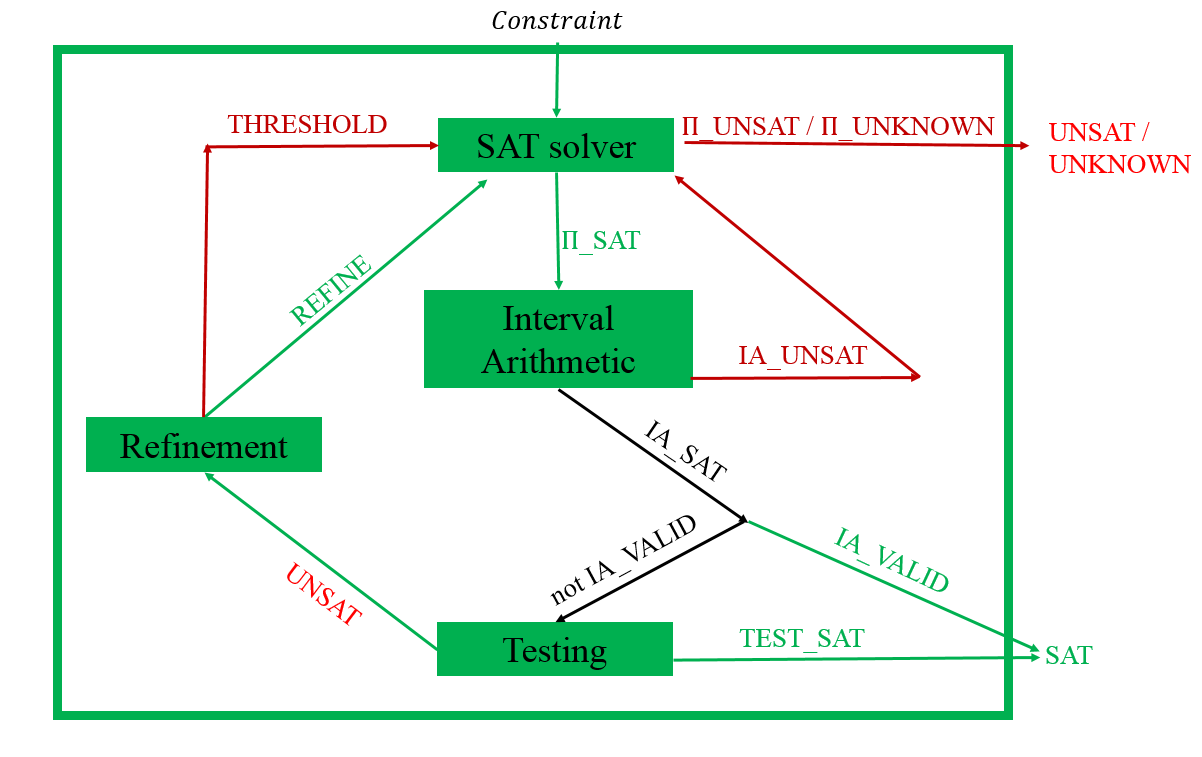
\includegraphics[width=\textwidth]{smt-design.png} 
\caption{\textbf{raSAT} design} 
\label{fig:smt-design} 
%\end{minipage}
\end{figure}

\begin{theorem} \label{theorem:terminating}
Starting with state $\Pi, \varphi, \emptyset, \emptyset, \varepsilon, \tau$, if $\Pi = \bigwedge\limits_{v_i \in V} v_i \in \langle l_i, h_i \rangle$ and $\{(x_1, x_2, \cdots) | \models_{\theta^I} \Pi, \theta = \{v_1 \mapsto x_1, v_2 \mapsto x_2, \cdots\} \}$ is bounded, raSATloop terminates.
\end{theorem}

\begin{proof}
In the worst case, all the interval will be decomposed into smallest boxes with size of $\varepsilon$ whose number are bounded to $\frac{h_1 - l_1}{\varepsilon}\frac{h_2 - l_2}{\varepsilon}\cdots$ (the number of variables in one polynomial constraint is also bounded). As a result, raSATloop terminates after checking all of these boxes.
\end{proof}

\section{Soundness - Completeness}
\subsection{Soundness}
\begin{theorem}
Let $(\Pi, \varphi, \mathring{\Pi}, \varphi^V, \varphi^U, \varepsilon, \tau)$ be any state of our system, then the following properties are invariants:
\begin{enumerate}
\item $\mathring{\Pi}_\mathbb{R} \subseteq T^p_\mathbb{R}$
\item $\varphi^V$ is $\mathring{\Pi}_{R}$-VALID.
\item $\varphi^U = \emptyset \vee (\varphi = \varphi^U \wedge \varphi^V)$
\item $\varphi$ is $\Pi_\mathbb{R}$-UNSAT $\implies$ $\varphi$ is $T^p_\mathbb{R}$-UNSAT
\end{enumerate}
\end{theorem}

\begin{proof}
\begin{enumerate}
\item Easy from the definition.
\item Easy to see.
\item Easy from the transitions.
\item The proof is done inductively:
\begin{itemize}
\item[$\bullet$] \sloppy Initial state: $(\bigwedge\limits_{v \in V}v \in (-\infty, +\infty), \varphi, \emptyset, \emptyset, \emptyset)$ and by definition, ${(\bigwedge\limits_{v \in V}v \in (-\infty, +\infty))_\mathbb{R} = T^p_R}$. Then, the invariant trivially holds.
\item[$\bullet$] Each transition is considered:
\begin{itemize}
\item For rules $\Pi$\_SAT, IA\_SAT the interval constraint $\Pi$ does not changed, so if the properties holds for the former state, it also does for the later one.
\item \sloppy For REFINE transition: \\ Denote ${\Pi' = \Pi \wedge (\neg I_j \vee I_{j1} \vee I_{j2}) \wedge (I_j \vee \neg I_{j1}) \wedge (I_j \vee \neg I_{j2}) \wedge (\neg I_{j1} \vee \neg I_{j2})}$. We will prove that $\varphi$ is $\Pi'_\mathbb{R}$-UNSAT $\implies \varphi$ is $\Pi_\mathbb{R}$-UNSAT. First suppose that $\varphi$ is $\Pi'_\mathbb{R}$-UNSAT. Let
\item for IA\_UNSAT transition, 
\end{itemize}
\end{itemize}
\end{enumerate}
\end{proof}

\begin{theorem}
Let $\varphi$ be the polynomial constraint to be solved. Starting with the state $(\Pi, \varphi, \emptyset, \emptyset, \emptyset)$, if our transitional system terminates and output:
\begin{itemize}
\item[$\bullet$] SAT then $\varphi$ is $T^p_\mathbb{R}$-SAT.
\item[$\bullet$] UNSAT then $\varphi$ is $T^p_\mathbb{R}$-UNSAT.
\end{itemize}
\end{theorem}

\begin{proof} We consider the SAT and UNSAT case.
\begin{enumerate}
\item If the system output SAT, there are two possibles transition to SAT:
\begin{itemize}
\item In the case of IA\_VALID, we have $\varphi^V$ is $\mathring{\Pi}_{R}$-VALID (invariant 2) $\implies \varphi^V$ is $\mathring{\Pi}_\mathbb{R}$-SAT $\implies \varphi$ is $\mathring{\Pi}_\mathbb{R}$-SAT (because $\varphi^V = \varphi$ is the condition of this transition). In addition, following invariant 1, we have $\mathring{\Pi}_\mathbb{R} \subseteq T^p_\mathbb{R}$, then $\varphi$ is $T^p_\mathbb{R}$-SAT (Lemma ~\ref{lemma:subtheory-SAT}).
\item \sloppy In the case of TEST\_SAT, $\varphi^U$ is $\mathring{\Pi}_\mathbb{R}$-SAT $\implies \exists M \in \mathring{\Pi}_\mathbb{R} \; \models_M \varphi^V$. Let ${M^c_\mathbb{R} \in \mathring{\Pi}_\mathbb{R}}$ such that $\models_{M^c_\mathbb{R}} \varphi^V$ which implies $(\varphi^V)^{M^c_\mathbb{R}} = 1$. In addition, because $\varphi^V$ is $\mathring{\Pi}_\mathbb{R}$-VALID (invariant 2) and $M^c_\mathbb{R} \in \mathring{\Pi}_\mathbb{R}$, we have $\models_{M^c_\mathbb{R}} \varphi^U$ or ${(\varphi^U)^{M^c_\mathbb{R}} = 1}$. Consider the evaluation of $\varphi$ under the model $M^c_\mathbb{R}$: ${(\varphi)^{M^c_\mathbb{R}} = (\varphi^U \wedge \varphi^V)^{M^c_\mathbb{R}}}$ (invariant 3) $= min((\varphi^U)^{M^c_\mathbb{R}}, (\varphi^V)^{M^c_\mathbb{R}}) = min(1, 1) = 1 \implies \models_{M^c_\mathbb{R}} \varphi \implies \varphi$ is $\mathring{\Pi}_\mathbb{R}$-SAT $\implies \varphi$ is $T^p_\mathbb{R}$-SAT (because of invariant 1 and Lemma ~\ref{lemma:IA-R-OP})
\end{itemize}
\item  If the system output UNSAT, there is only one transition of rule $\Pi$\_UNSAT. Because $\Pi \models_{SAT} \bot$, $\Pi_\mathbb{R}$ is empty (Lemma ?). As a result, $\varphi$ is $\Pi_\mathbb{R}$-UNSAT which implies that $\varphi$ is $T^p_\mathbb{R}$-UNSAT (invariant 4).
\end{enumerate}
\end{proof}

\subsection{Completeness}
\begin{definition} \label{def:OT-complete}
\sloppy
Let $\Pi = \bigwedge\limits_{v \in V} v \in i$ with $i \in \mathbb{I}$, and ${\varphi = \bigwedge\limits_{i=1}^n f_i > 0}$. An over-approximation $T^p_O$ of $T^p_\mathbb{R}$ is complete if for each open set ${O \subset \{(r_1,r_2,\cdots) |  \models_{\theta^\mathbb{I}} \Pi; \theta = \{v_i \mapsto r_i \in \mathbb{R} | v_i  \in V\}\}}$, we have ${\forall c \in O; \; \forall \delta > 0; \; \exists \gamma > 0; \; (\langle c - \gamma, c + \gamma \rangle \in O \text{ and } \models_{\Pi'^p_\mathbb{R}} \bigwedge\limits_{i=1}^n(f_i(c)-\delta < f_i(x) < f_i(c) + \delta)}$ where ${\Pi' = \bigwedge\limits_{v_i \in V} v_i \in \langle c_i - \gamma, c_i + \gamma \rangle}$, and ${c = (c_1, c_2, \cdots)}$
\end{definition}

\begin{lemma} \label{lem:sat-complete}
Let $\Pi = \bigwedge\limits_{v_i \in V} v_i \in \langle l_i, h_i \rangle$ where $\langle l_i, h_i \rangle \in \mathbb{I}$ is bounded; and ${\varphi = \bigwedge\limits_{j = 1}^n f_j > 0}$. Denote $S = \{(x_1, x_2, \cdots) | \theta = \{v_i \mapsto x_i | v_i \in V \}; \models_{\theta^I} \Pi \text{ and } \models_{\theta^p_\mathbb{R}}\varphi \}$. If $S \neq \emptyset$ and $\{(v_1, v_2, \cdots) | v_1 \in (l_1, h_1), v_2 \in (l_2, h_2) \cdots \}$ is open, then $S$ contain an open set.
\end{lemma}

\begin{proof}
\sloppy
Because $S \neq \emptyset$, there exist $c = (c_1, c_2, \cdots) \in S$. By definition of $S$, ${\forall j \in \{1, \cdots, n\} f_j(c) > 0}$. Take $\delta = \min\limits_{j=1\cdots n} f_j(c)$, then $\delta > 0$. Because the polynomials are continuous, there exists $\gamma > 0$ such that $\forall v \in \langle c - \gamma, c + \gamma \rangle; \; \bigwedge\limits_{j=1}^n f_j(c) - \delta < f_j(v) < f_j(c) + \delta$ which implies ${\forall v \in \langle c - \gamma, c + \gamma \rangle; \; \bigwedge\limits_{j=1}^n f_j(v) > 0}$ (because $\delta = \min\limits_{j=1\cdots n}f_j(c) \le f_j(c)$) for any $j$.
Now consider the open interval $O = \{(x_1, x_2, \cdots) | x_1 \in getIntv(c_1, l_1, h_2, \delta), \cdots \}$ where $getIntv(c, l, h, \delta)$ is defined as following:
\begin{center}
$getIntv(c, l, h, \delta) = $
\end{center}
\end{proof}


\begin{theorem} \label{theorem:SAT-complete}
Let $\Pi = \bigwedge\limits_{v_i \in V} v_i \in \langle l_i, h_i \rangle$ where $\langle l_i, h_i \rangle \in \mathbb{I}$ is bounded; and ${\varphi = \bigwedge\limits_{j = 1}^n f_j > 0}$. Denote $S = \{(x_1, x_2, \cdots) | \theta = \{v_i \mapsto x_i | v_i \in V \}; \models_{\theta^I} \Pi \text{ and } \models_{\theta^p_\mathbb{R}}\varphi \}$. If $S \neq \emptyset$ and $\{(v_1, v_2, \cdots) | v_1 \in (l_1, h_1), v_2 \in (l_2, h_2) \cdots \}$ is open, then raSATloop can detect the satisfiability of $\varphi$ with assumption that IA is complete.
\end{theorem}


\begin{proof}
Based on Lemma~\ref{lem:sat-complete}, there exist an open box $(l, h)$ such that $\forall (x_1, x_2, ...) \in (l, h); \; \bigwedge\limits_{j=1}^n f_j > 0 $. Take any $c \in (l, h)$ and take $\delta = \min\limits_{j = 1\cdots n}(f_j(c))$. Because IA is complete by assumption, from Definition~\ref{def:OT-complete} there exists $\gamma > 0$ such that $\langle c - \gamma, c + \gamma \rangle \in (l, h)$ and $\bigwedge\limits_{j = 1}^n f_j(c) - \delta < f_j(v) < f_j(c) + \delta$ is ${\bigwedge\limits_{v_i \in V}v_i \in \langle c_i - \gamma, c_i + \gamma \rangle}^p_{IA}$-VALID. By taking this $\gamma$ as the threshold in $(\Pi, \varphi, \emptyset, \emptyset, \varepsilon, \bot)$, raSATloop will terminate (Theorem~\ref{theorem:terminating}). Furthermore, $\langle c - \gamma, c + \gamma \rangle \in (l, h) \implies (c + \gamma) - (c - \gamma) < h - l \implies 2\gamma < h - l$. As a consequence, decomposition eventually creates a box of size $\gamma$ inside $(h, l)$ which can be used to conclude the validity of the constraint by IA.
\end{proof}


\begin{theorem} \label{theorem:UNSAT-complete}
\sloppy
Let $\Pi = \bigwedge\limits_{v_i \in V} v_i \in \langle l_i, h_i \rangle$ where $\langle l_i, h_i \rangle \in \mathbb{I}$ is bounded; and ${\varphi = \bigwedge\limits_{j = 1}^n f_j > 0}$. Denote $S_j = \{(x_1, x_2, \cdots) | \theta = \{v_i \mapsto x_i | v_i \in V \};\models_{\theta^I} \Pi \text{ and } \models_{\theta^p_\mathbb{R}}f_j \}$. If $\bigcap\limits_{j = 1}^nclosure(S_j) = \emptyset$, then raSATloop can prove the unsatisfiability of $\varphi$ with assumption that IA is complete.
\end{theorem}


\begin{proof}
\sloppy
Let $f(v) = \min\limits_{j = 1}^nf_j(v)$, then $f(v)$ is continuous. Because ${D = \{(x_1, x_2, \cdots) | \theta = \{v_1 \mapsto x_1, v_2 \mapsto x_2, \cdots\}; \models_{\theta^I} \Pi\}}$ is compact, ${\delta = |\max\limits_{v \in D}f(v)}|$ exists. First we will prove that $\delta > 0$. In fact, suppose $\delta = 0 \implies \forall c \in D; \; f(c) = 0 \implies \forall c \in D \forall j \in \{1, \cdots, n\}f_j(c) \ge 0$. This contradicts with the assumption that $\bigcap\limits_{j = 1}^nclosure(S_j) = \emptyset$.

Because IA is complete, by Definition~\ref{def:OT-complete}, for any point $c \in D$, there exists $\gamma > 0$ such that $\langle c - \gamma, c + \gamma \rangle \in D$ and $\bigwedge\limits_{j = 1}^n f_j(c) - \delta < f_j(v) < f_j(c) + \delta$ is ${\bigwedge\limits_{v_i \in V}v_i \in \langle c_i - \gamma, c_i + \gamma \rangle}^p_{IA}$-VALID. Consider $f_k(c) = \min\limits_{j=1}^nf_j(c)$ then $f_k(c) < 0$ otherwise a contradiction with the assumption that $\bigcap\limits_{j = 1}^nclosure(S_j) = \emptyset$ exists. In addition by definition of $f(v)$ we have $f_k(c) = f(c) \le \max\limits_{v \in D}f(v) \implies f_k(c) + \delta < 0 \implies \bigwedge\limits_{j = 1}^n f_j(v) > 0$ is UNSAT over $\bigwedge\limits_{v_i \in V}v_i \in \langle c_i - \gamma, c_i + \gamma \rangle$. For any point in $D$, we can find a small box so that the constraint is unsatisfiable. If $\varepsilon$ is small enough, the unsatisfiability can be detected by raSATloop.
\end{proof}


\begin{comment}
\section{Over-Approximation Theory Refinement}
\label{sec:soundness}

From now on, We focus on a \emph{polynomial inequality} such that 
$I_i$ and $\psi_j(x_1,\cdots,x_n)$ are an open interval $(a_i,b_i)$ and 
an atomic polynomial inequaltiy (API) $f_j > 0$, respectively. 
We denote $\mathbb{S}(f_j) = \{x \in \Real^n \mid f_j > 0 ~\text{holds}\}$.

For ICP, it is folklore that, for polynomial inequality 
$\exists x_1 \in (a_1,b_1) \cdots x_n \in (a_n,b_n) . \wedge_{i} f_i > 0$, 
\begin{itemize}
\item if $\exists x_1 \in (a_1,b_1) \cdots x_n \in (a_n,b_n) . \wedge_{i} f_i > 0$ is SAT, 
ICP eventually detects it, and 
\item if $\exists x_1 \in [a_1,b_1] \cdots x_n \in [a_n,b_n] . \wedge_{i} f_i \geq 0$ is UNSAT, 
ICP eventually detects it, 
\end{itemize}
under the assumptions of {\em fair} decomposition and bounded intervals $(a_i,b_i)$. 
We will prepare terminology and briefly review this fact. 

%%%%%%%%%%%%%%%%%%%%%%
\suppress{
\begin{definition} \label{def:poly}
A polynomial inequality is a bounded quantification 
$\exists x_1 \in I_1 \cdots x_n \in I_n. \psi(x_1,\cdots,x_n)$ 
such that 
\begin{itemize}
\item each $I_i$ is an open interval $x_i \in (a_i,b_i)$, and 
\item $\psi(x_1,\cdots,x_n)$ is a conjunction of $f_j > 0$ 
where $f_j$ is a polynomial over $\{x_1, \cdots, x_n\}$. 
\end{itemize}
$f_i > 0$ is called an atomic polynomial inequality (API). 
We denote $\mathbb{S}(F) = \{x \in \Real^n \mid F ~\text{holds}\}$.
\end{definition}

\begin{example} \label{examp:poly_ieq}
$\exists x \in (-1,3)~y \in (2,4) . (x^3y - y^4 > 0) \wedge (y^3 -xy >0)$
is an example of a polynomial inequality with 2 variables and 2 APIs. 
\end{example}
}
%%%%%%%%%%%%%%%%%%%%%%

\begin{definition}
An \emph{open box} of dimension $n$ is a set $(a_1,b_1) \times \cdots \times (a_n,b_n)$ 
where $a_i, b_i \in \Real, a_i \leq b_i$.  
For $\mathfrak{a} = (a_1, \cdots, a_n)$ and $\mathfrak{b} = (b_1, \cdots, b_n)$, 
we denote $(a_1,b_1) \times \cdots \times (a_n,b_n)$ by $(\mathfrak{a}, \mathfrak{b})$. 
\end{definition}

The set of all open boxes is a basis of Euclidean topology on $\Real^n$. 
In $\Real^n$, a set $U$ is compact if, and only if, $U$ is a bounded closed set. 
We denote a closure of a set $U$ by $\overline{U}$. 
%
Since a polynomial is continuous, 
$\mathbb{S}(\bigwedge \limits_{i=1}^m f_i > 0)$ is an open set. 
Note that $\Rat$ is dense in $\Real$, and an SAT instance in reals can be replaced with one in rationals. 

%%%%%%%%%%%%%%%%%%%%%%%%%%%%%%
\suppress{
\begin{lemma} \label{cor:rattoreal}
For a polynomial inequality
$F = \exists x_1 \in I_1 \cdots x_n \in I_n. \bigwedge \limits_{j=1}^m f_j > 0$, 
If there exists an SAT instance of F in $\Real^n$, there exists also in $\Rat^n$. 
\end{lemma}

\begin{lemma} \label{cor:refinement}
Suppose that $a_j < b_j$ for $1 \leq j \leq n$ and $f_i$'s are polynomials. 
Assume $a_k < c < b_k$ for some $k$. 
Then, 
$\exists x_1 \in (a_1,b_1) \cdots x_n \in (a_n,b_n). \bigwedge \limits_{i=1}^m f_i > 0$ 
is SAT (resp. UNSAT) if, and only if, 
$\exists x_1 \in (a_1,b_1) \cdots x_k \in (a_k,c) \cdots x_n \in (a_n,b_n). 
 \bigwedge \limits_{i=1}^m f_i > 0 
 \vee 
 \exists x_1 \in (a_1,b_1) \cdots x_k \in (c,b_k) \cdots x_n \in (a_n,b_n)). 
 \bigwedge \limits_{i=1}^m f_i > 0$ 
is SAT (resp. UNSAT). 
\end{lemma}

\begin{pf}
We show for the SAT case. If-part is obvious. For only-if-part, 
since $\mathbb{S}(\bigwedge \limits_{i=1}^m f_i > 0)$ is an open set, 
if $y \in (a_1,b_1) \times \cdots \{c\} \cdots \times (a_n,b_n)$ satisfies 
$\bigwedge \limits_{i=1}^m f_i > 0$, 
there exists $x_1 \in (a_1,b_1) \cdots x_k \in (a_k,c) \cdots x_n \in (a_n,b_n)$
(also $x_1 \in (a_1,b_1) \cdots x_k \in (c,b_k) \cdots x_n \in (a_n,b_n)$) that satisfies
$\bigwedge \limits_{i=1}^m f_i > 0$. 
\end{pf}

Lemma~\ref{cor:rattoreal} says that proving SAT of $F$ in $\Real$ is reduced to 
that in $\Rat$. 
Lemma~\ref{cor:refinement} says that, in the refinement step, we can apply refinement 
$x_k \in (a_k,b_k)$ to $x_k \in (a_k,c) \vee x_k \in (c,b_k)$, 
instead of $x_k \in (a_k,c] \vee x_k \in (c,b_k) $
(i.e., $c$ is ignored). 
}
%%%%%%%%%%%%%%%%%%%%%%%%%%%%%%

Initially, interval constraints consists of conjunction only. Later, by refinements, it becomes a CNF. 


%\begin{example} \label{examp:poly_ieq}
$\exists x \in (-1,3)~y \in (2,4) . (x^3y - y^4 > 0) \wedge (y^3 -xy >0)$
is an example of a polynomial inequality with 2 variables and 2 APIs. 

For instance, $x \in (-1,3)$ and $y \in (2,4)$ are refined to smaller intervals
such that 
$\exists x \in (-1,1) y \in (2,4) . (x^3y - y^4 > 0) \wedge (y^3 -xy >0) \vee 
 \exists x \in (1,3) y \in (2,4) . (x^3y - y^4 > 0) \wedge (y^3 -xy >0)$, 
which results a CNF 
$(x \in (-1,1) \vee x \in (1,3)) \wedge (y \in (2,4)) \wedge (x^3y - y^4 > 0) \wedge (y^3 -xy >0)$.
%(only the CNF formula $(x \in (-1,1) \vee x \in (1,3)) \wedge (y \in (2,4))$ is given to SAT solver).
%\mizuhito{could you fulfill? Direct encoding seems a DNF?}. 
%\end{example}

Note that an interval arithmetic used in ICP is a converging theory. 

\begin{definition} \label{def:completeOT}
Let
$F = \exists x_1 \in I_1 \cdots x_n \in I_n. \bigwedge \limits_{j=1}^m f_j > 0$
be a polynomial inequality such that each $I_i$ is bounded. 
An over-approximation theory $O.T$ is {\em converging} 
if, for each $\delta > 0$ and $c = (c_1, \cdots, c_n) \in I_1 \times \cdots \times I_n$, 
there exists $\gamma > 0$ such that 
$\bigwedge \limits_{j=1}^n x_j \in (c_j - \gamma, c_j + \gamma) \models_{O.T} 
 \bigwedge \limits_{i=1}^m (f_i(c) - \delta < f_i(x) < f_i(c) + \delta)$. 
\end{definition}

$O.T$ refinemnet loop is shown in Fig.~\ref{fig:OTrefine}~(a). 
A standard ICP based algorithm of an SMT solver applies it with $O.T$ as a classical interval arithemtic. 
The variation of interval arithemtic will be presented in Section~\ref{sec:approximation}. 
\begin{figure}[ht]
\begin{minipage}[b]{1.0\linewidth}
\centering
\begin{tabular}{c@{\quad}c}
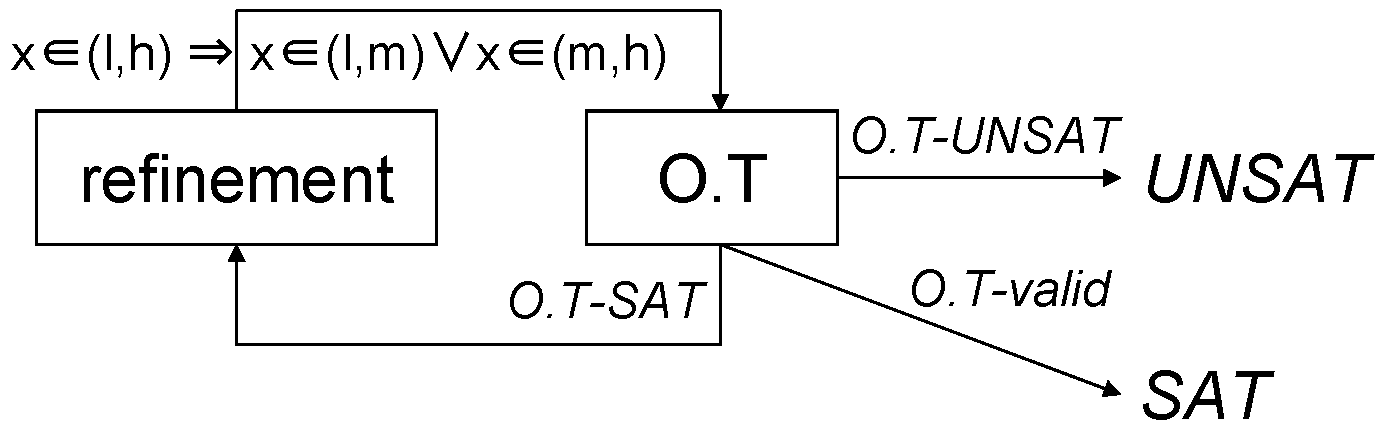
\includegraphics[height=0.6in,width=1.7in]{OTloop.png} & 
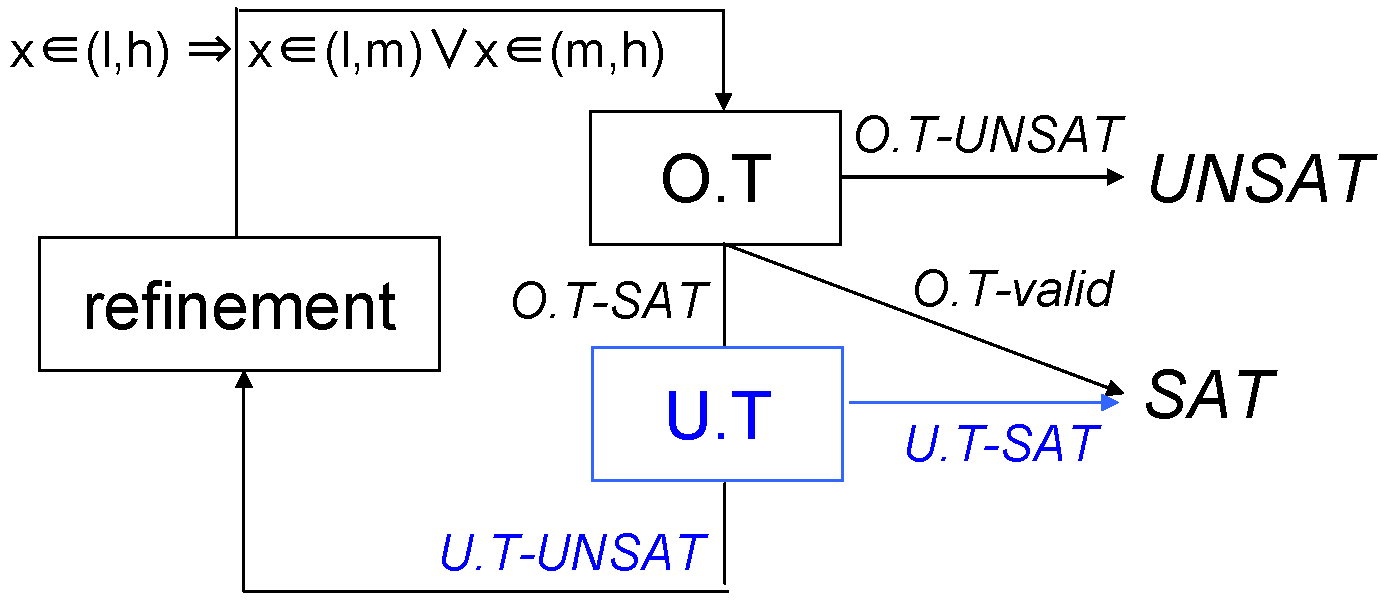
\includegraphics[height=0.9in,width=1.7in]{rasatloop.png} \\   
\mbox{(a) $O.T$ refinement loop} & \mbox{{\bf raSAT} loop} \\
\end{tabular}
\end{minipage} 
\caption{Rfinement loops} 
\label{fig:OTrefine} 
\end{figure}


\begin{definition} 
Let
$F = \exists x_1 \in I_1 \cdots x_n \in I_n. \bigwedge \limits_{j=1}^m f_j > 0$
for $I_i = (a_i,b_i)$.
A refinement strategy is {\em fair}, if, for each $c_j \in (a_j,b_j)$ and $\gamma > 0$, 
a decomposition of $I_i$ for each $i$ eventually occurs in $(c_j - \gamma, c_j + \gamma)$ 
(as long as neither SAT nor UNSAT is detected). 
\end{definition}

\begin{theorem} \label{theorem:RelComp}
Let
$F = \exists x_1 \in I_1 \cdots x_n \in I_n. \bigwedge \limits_{j=1}^m f_j > 0$
for $I_i = (a_i,b_i)$.
Assume that an over-approximation theory $O.T$ is converging, 
each $(a_i,b_i)$ is bounded, and a refinement strategy is fair. 
Then, 
\begin{itemize}
\item if $\exists x_1 \in (a_1,b_1) \cdots x_n \in (a_n,b_n) . \wedge_{i} f_i > 0$ is SAT, 
$O.T$ refinemnet loop eventually detects it, and
\item if $\exists x_1 \in [a_1,b_1] \cdots x_n \in [a_n,b_n] . \wedge_{i} f_i \geq 0$ is UNSAT, 
$O.T$ refinement loop eventually detects it.  
\end{itemize}
\end{theorem}


\begin{proof} 
The former is proved by the fact that, if $F$ is SAT, there exists a non-empty neiborhood (open box) 
in $\cap~\mathbb{S}(f_j)$. 
If the box decomposition strategy is fair, the refinemnet will eventually find such an open box. 

For the latter, assume that 
$\overline{F} = \exists x_1 \in [a_1,b_1] \cdots x_n \in [a_n,b_n] . \wedge_{i} f_i \geq 0$ is UNSAT. 
Thus, $\cap~\overline{\mathbb{S}(f_i)} = \emptyset$. 
Let $\delta_{j,k} = min \{|f_j(\bar{x}) - f_k(\bar{x})| \mid \bar{x} \in I_1 \times \cdots \times I_n\}$. 
Since $f_i$'s are continuous and $\overline{I_i}$'s are compact, $\delta_{j,k}$ is well defined,
and $\delta_{j.k} > 0$ for some $j,k$. 
Let $\delta = \frac{min \{ \delta_{j,k} \}}{2}$. 
Since $O.T$ is converging, there exists $\gamma > 0$ for $\delta > 0$ 
satisfying Definition~\ref{def:completeOT}, and fair decomposition eventually finds open boxes
such that $\mathbb{S}(f_j)$ and $\mathbb{S}(f_k)$ are separated. 
%\qed
\end{proof}

Limitations for detecting UNSAT occur on \emph{kissing} and \emph{convergent} cases. 
Fig.~\ref{fig:limit} left shows a kissing case 
$x^2 + y^2 < 2^2 \wedge (x-4)^2 + (y-3)^2 < 3^2$ such that 
$\overline{\mathbb{S}(- x^2 - y^2 + 2^2)} \cap \overline{\mathbb{S}(- (x-4)^2 - (y-3)^2 + 3^2)} 
= \{(x,y) \mid (1.6, 1.2)\}$. 
Thus, there are no coverings to separate them. 
%$x^2 + y^2 < 2^2$ and $(x-4)^2 + (y-3)^2 < 3^2$. 
%
Fig. \ref{fig:limit} right shows a convergent case 
$y > x + \frac{1}{x} \wedge y < x \wedge x > 0$, which is equivalent to 
$xy > x^2 + x \wedge y < x \wedge x > 0$. 
%The open box is $(0,\infty) \times (0,\infty)$ and 
There are no finite coverings to separate them. 
%$y > x + \frac{1}{x}$ and $y < x$ for $x > 0$. 

\begin{figure}[ht]
%\begin{minipage}[b]{1.0\linewidth}
\centering
\begin{tabular}{cc}
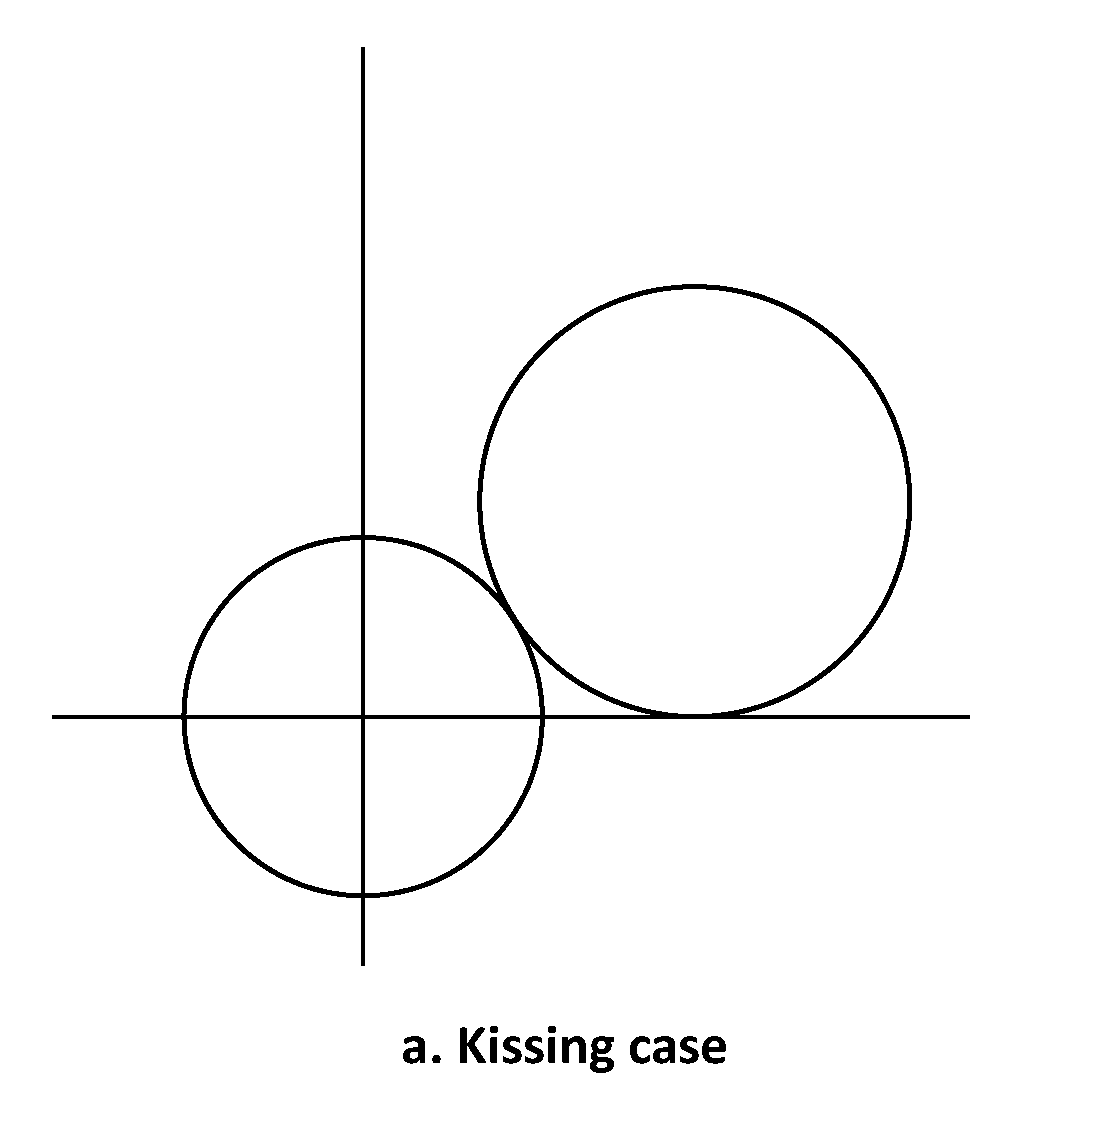
\includegraphics[height=1.65in,width=1.7in]{kissing.eps} &
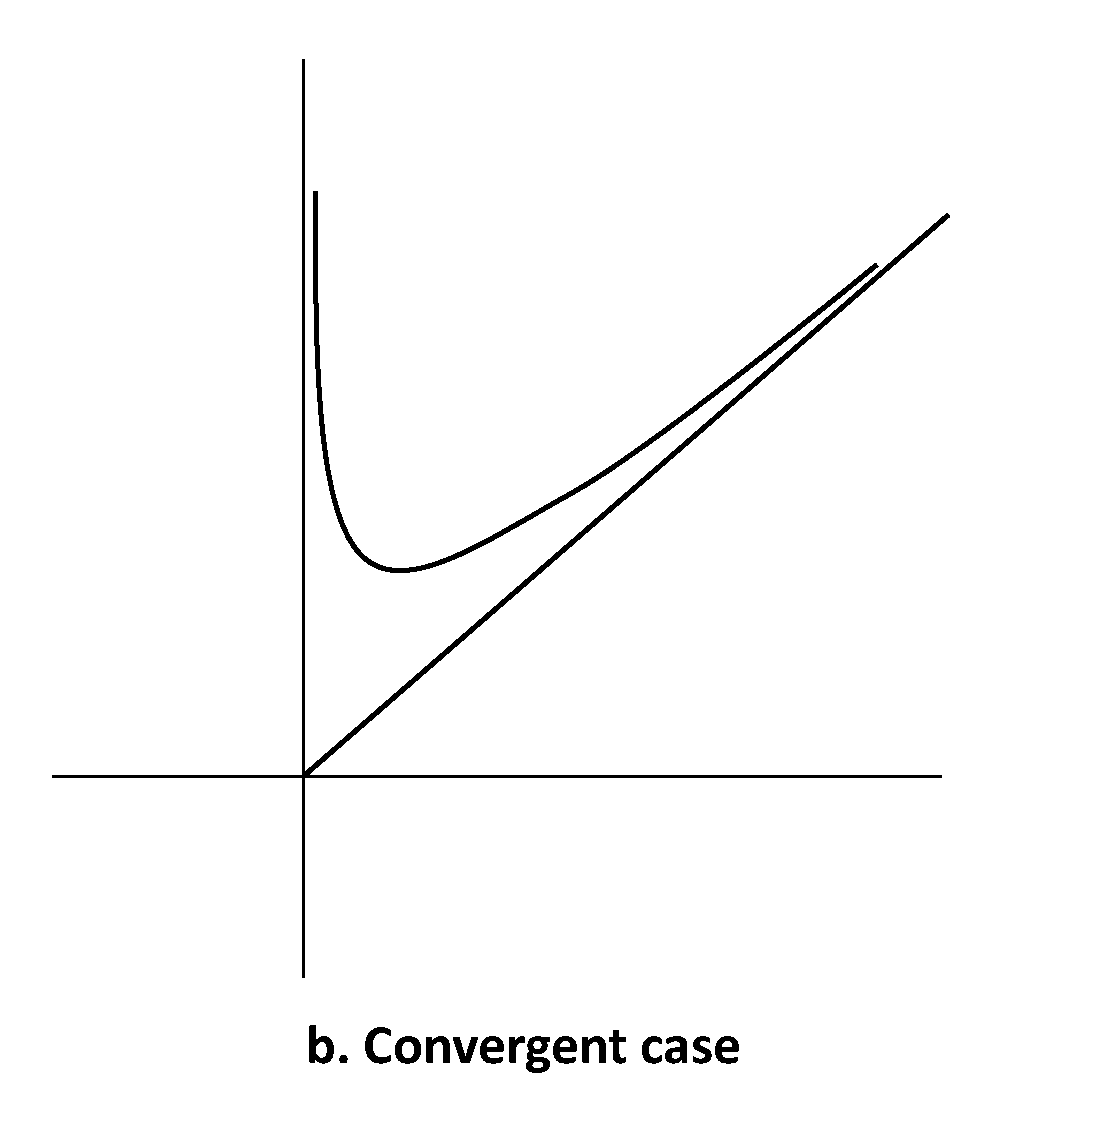
\includegraphics[height=1.65in,width=1.7in]{convergence.eps}
\end{tabular}
\caption{Limitations for proving UNSAT} 
\label{fig:limit} 
%\end{minipage}
\end{figure} 
\end{comment}